\documentclass[a4paper, 10pt, conference]{ieeeconf}      % Use this line for a4 paper

\usepackage{FG2019}
\usepackage[utf8]{inputenc}
\usepackage[french]{babel}
\usepackage[T1]{fontenc}
\usepackage{caption}
\usepackage{graphicx}


\FGfinalcopy % *** Uncomment this line for the final submission



\IEEEoverridecommandlockouts  % This command is only needed if you want to use the \thanks command
\overrideIEEEmargins
% See the \addtolength command later in the file to balance the column lengths
% on the last page of the document

% The following packages can be found on http:\\www.ctan.org
%\usepackage{graphicx} % for pdf, bitmapped graphics files
%\usepackage{epsfig} % for postscript graphics files
%\usepackage{mathptmx} % assumes new font selection scheme installed
%\usepackage{times} % assumes new font selection scheme installed
%\usepackage{amsmath} % assumes amsmath package installed
%\usepackage{amssymb}  % assumes amsmath package installed

\def\FGPaperID{****} % *** Enter the FG 2019 Paper ID here

\title{\LARGE \bf IA : Real time emotion recognition on video }

%use this in case of a single affiliation
%\author{\parbox{16cm}{\centering
%    {\large Huibert Kwakernaak}\\
%    {\normalsize
%    Faculty of Electrical Engineering, Mathematics and Computer Science, University of Twente, Enschede, The Netherlands\\}}
%    \thanks{This work was not supported by any organization.}% <-this % stops a space
%}

%use this in case of several affiliations
\author{\parbox{16cm}{\centering
    {\large Romain Daussaint \& Lucas Honnay}\\
    {\large Advisor : Dr. Rim Slama - rim.slama@henallux.be}\\
    {\normalsize
    Industrial Engineering Departement, Henallux College\\
	Rue d’Arlon, 112,  B-6760 Virton
    }}}

\begin{document}

\ifFGfinal
\thispagestyle{empty}
\pagestyle{empty}
\else
\author{Anonymous FG 2019 submission\\ Paper ID \FGPaperID \\}
\pagestyle{plain}
\fi
\maketitle


%%%%%%%%%%%%%%%%%%%%%%%%%%%%%%%%%%%%%%%%%%%%%%%%%%%%%%%%%%%%
\begin{abstract}

As part of the intelligent systems course in the first year of the Master's program, we had to develop an application that uses artificial intelligence recognition for a part of the human body.
We choose to make one which detects live facial recognition of emotions via the webcam of the user's computer.

\end{abstract}


%%%%%%%%%%%%%%%%%%%%%%%%%%%%%%%%%%%%%%%%%%%%%%%%%%%%%%%%%%%%
\section{INTRODUCTION}

Many sectors are interested in automating the recognition of emotions.
These applications are related to many fields like marketing for applications to measure customer satisfaction, predict products that interest them, evaluate the reactions of users on a website or improve recommendations systems.
But also in the transport sector to detect worrying signs in the driver, in medicine, in security or even in education.\

So the goal of this project is to take a ten second video of the user by his webcam.
Then calculate and show the average of each of the seven common emotions (sad, happy, neutral, disgust, fear, angry and surprise) the user made during these ten seconds, and bring to light the dominant emotion.


%%%%%%%%%%%%%%%%%%%%%%%%%%%%%%%%%%%%%%%%%%%%%%%%%%%%%%%%%%%%
\section{STATE OF THE ART}
Several projects have already been carried out on emotion recognition, we show you below some of these projects that we consulted:\\
\scriptsize NB: You will find the source of each point in the references at the end of the article.\\
	
\normalsize
$^1$The first one is a TFE about emotion recognition by image processing. It helps us to understand how to detect an emotion and what are the characteristics of a happy, disgusted, sad face, etc.\\

$^2$The second one is a little presentation on how the system works for the emotion recognition (model, database,…).\\

$^3$The third one is an example of a program for the realisation of an emotion recognition in a git hub repository.\\

$^4$We also used an article explaining a program to perform real time emotion recognition.\\

$^5$Finally, we read a video of someone explaining the basics of the CNN and how to standardise the data, create a model and train it.

\addtolength{\textheight}{-3cm}   % This command serves to balance the column lengths on the last page of the document manually. It shortens the textheight of the last page by a suitable amount. This command does not take effect until the next page so it should come on the page before the last. Make sure that you do not shorten the textheight too much.

%%%%%%%%%%%%%%%%%%%%%%%%%%%%%%%%%%%%%%%%%%%%%%%%%%%%%%%%%%%%
\section{OUR SOLUTION}
In this section we are going to explain our model and the interface we choose to run the application.

\subsection{Network architecture}
To make it possible we used the deep learning and we headed for the CNN model (Convolutional Neural Network).
Indeed, CNN is used a lot for facial recognition or image classification, so we decided to use this technology for our project.\\
The CNN works like this:
\begin{itemize}
\item The convolution applies a filter to the input image.
\item The filter parameters are learned through the learning.
\item A learnt filter will be able of detecting features in an image; for example, angles, and use them to classify at best the image.
\end{itemize}

The process learning is done with convolution layers on images from a database of many faces with different emotion. The output will be the emotion that the process will have found.\\
In the image below, we can see an example of the architecture of a CNN model.
You can see the input image, the feature learning with the convolution and pooling funtions and then the classification that attribute a class to the image, in this case a car, a truck, a van...

\begin{center}
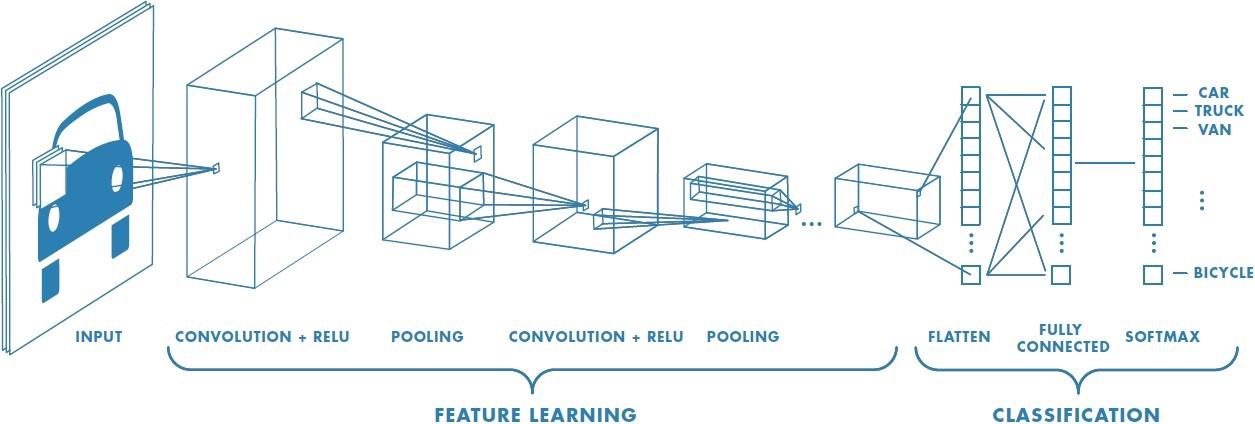
\includegraphics[scale=0.17]{Exemple_CNN.jpeg}
\captionof{figure}{CNN Example}
\label{fig1}
\end{center}

To design our CNN model for emotion detection we use 3 different layers:
the first convolution layer contains 64 neurons with ReLu function as an activation function and a dropout function to make learning efficiently.
Dropout offers a remarkably effective regularization method to reduce overfitting.
The $"0.5"$ that we use in this function correspond to a $0.5$ multiplication of the neurons from the previous layers.\\
The parameters of the second convolution layer are the same that the first layer.
And the third convolution layer contains 128 neurons also with a ReLu as an activation function.
Then after the convolution layers we flatten the data to a 1D matrix and we realised the probability of the 7 classes for each emotion thanks to the softmax function.
So, with this function it's possible to have the probability of each emotion for one input.

\begin{center}
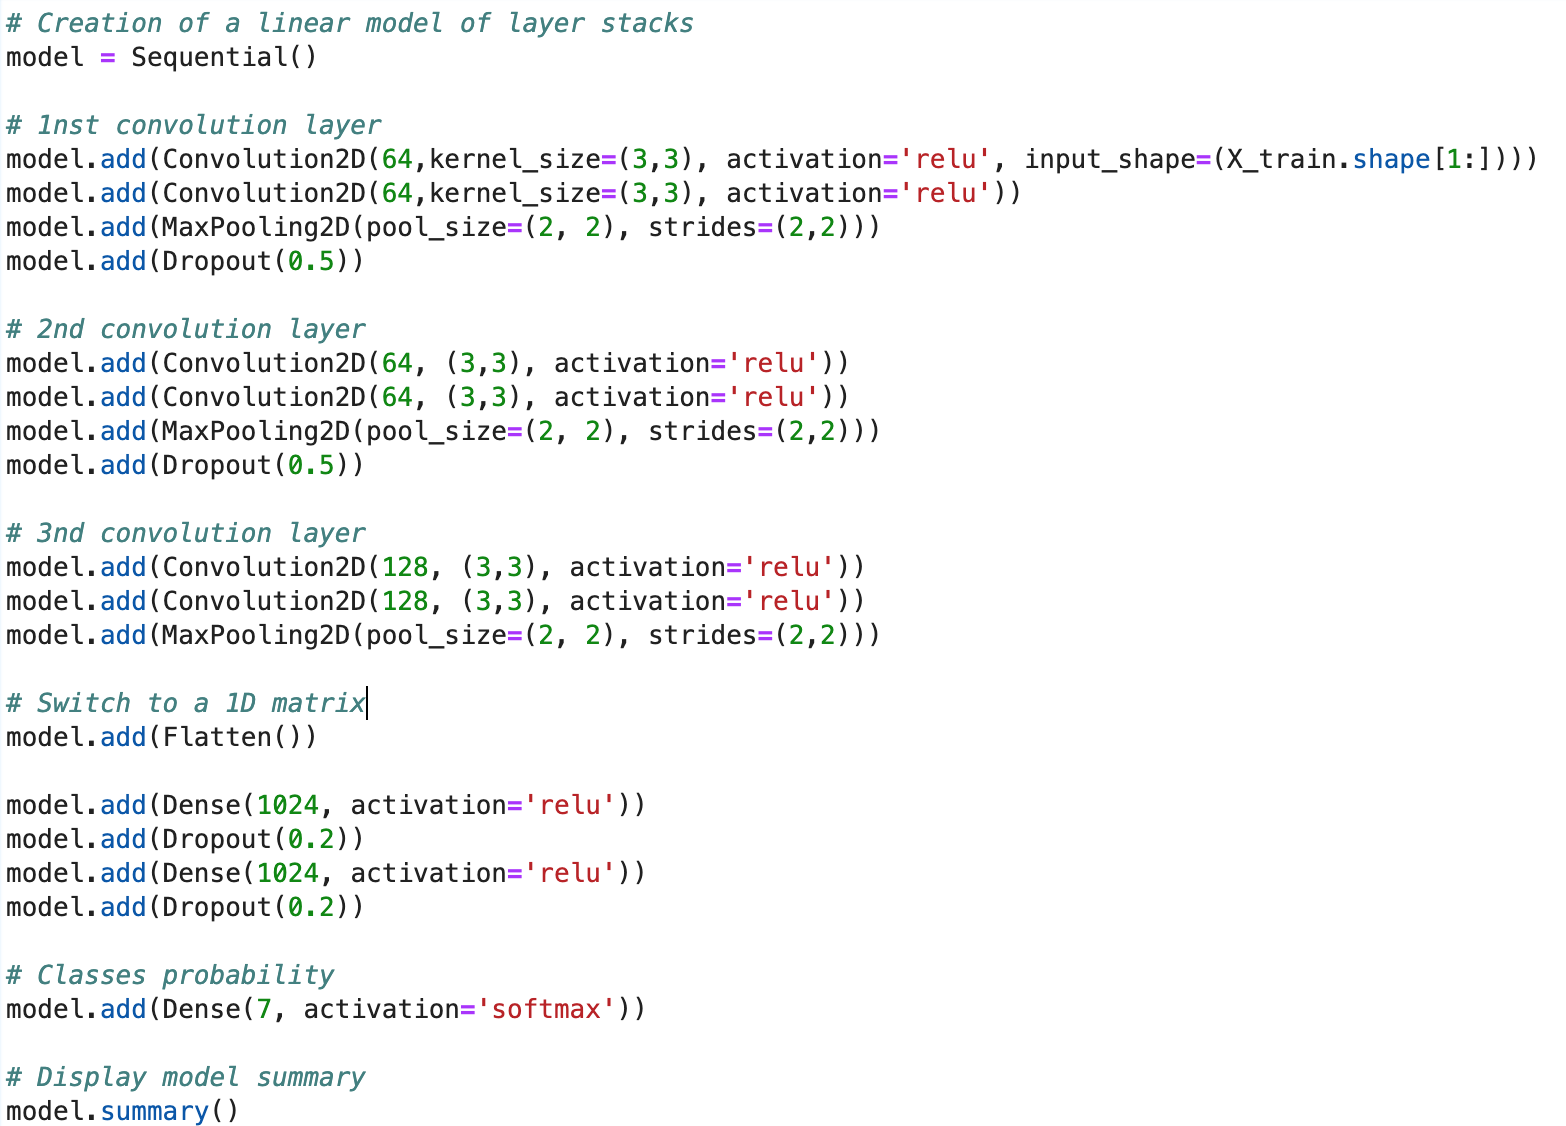
\includegraphics[scale=0.3]{Model}
\captionof{figure}{Model convolution layers}
\label{fig2}
\end{center}


Then, concerning the batch size, we use a batch size of 64.
With a batch size of 64 and a database containing 28709 training samples we have a batch size of 449.
The algorithm takes the first 449 samples (from the 1st to the 449th) of the training data set and trains the network.
Then it takes the remaining 449 samples (449th to 898th) and trains the network again.
We can continue this procedure until we have propagated all the samples through the network.

\subsection{Interface conception and design}
To simulate our project, we created an interface with Tkinter.
The configuration of the window, the buttons and the texts are also done with Python on our notebook.

\begin{center}
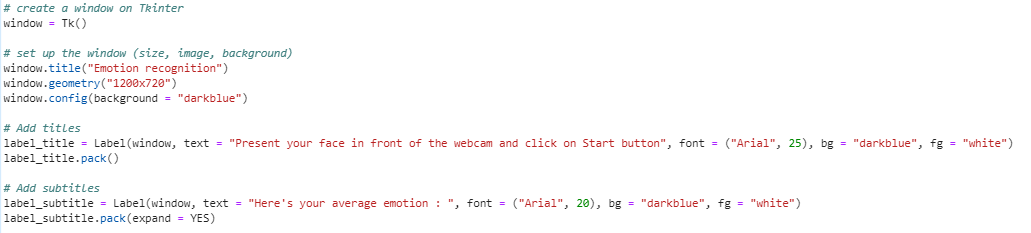
\includegraphics[scale=0.3]{Model1}\\
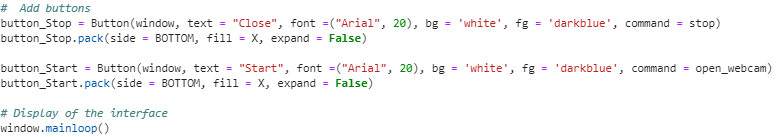
\includegraphics[scale=0.4]{Model2}
\captionof{figure}{Interface code}
\label{fig3}
\end{center}

In the previous image you can see part of the code to:
\begin{itemize}
\item Create a window on Tkinter
\item Set up the window (size, image, background)
\item Add titles and subtitles
\item Add buttons
\end{itemize}\

On the next picture you can see the result of this code and the design of our application :

\begin{center}
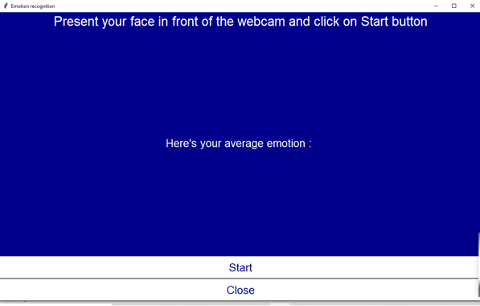
\includegraphics[scale=0.7]{Interface}
\captionof{figure}{Interface welcome page}
\label{fig4}
\end{center}

To start the emotion recognition, you have to click on the start button. At this moment the camera is opening and you present your face in front of the objective.

\begin{center}
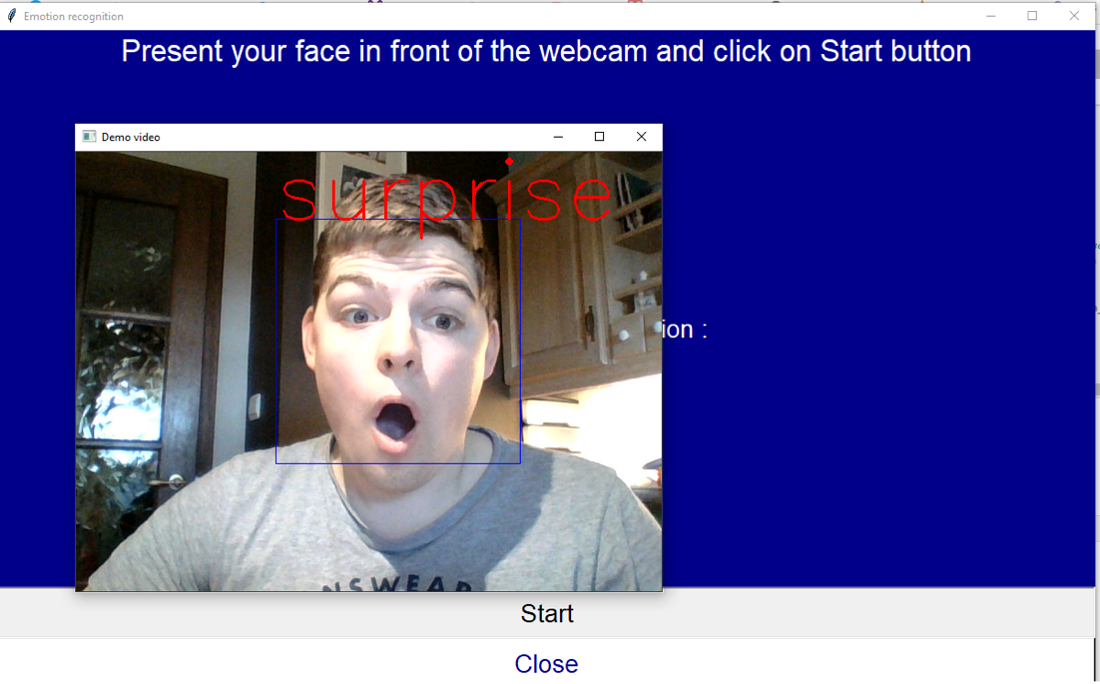
\includegraphics[scale=0.7]{Interface1}
\captionof{figure}{Direct reading emotion}
\label{fig5}
\end{center}

The program will detect and display your emotion in real time.
After a delay of 10 seconds the camera will cut off and an average of your emotions will be displayed in the interface.
Also, your dominant emotion will be displayed in the interface.

\begin{center}
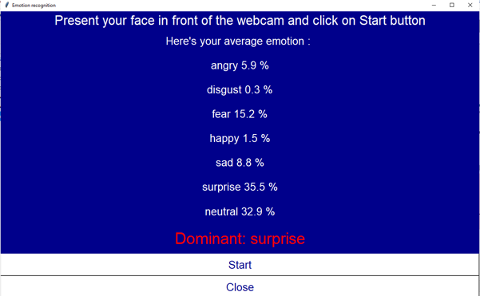
\includegraphics[scale=0.7]{Interface2}
\captionof{figure}{Application results}
\label{fig6}
\end{center}

If you want to restart the recognition of emotions, you have to click on start. If you want to close the application, you have to click on the close button.

%%%%%%%%%%%%%%%%%%%%%%%%%%%%%%%%%%%%%%%%%%%%%%%%%%%%%%%%%%%%
\section{EXPERIMENTS}
In this section we will explain the database, we used and the results we obtained from our CNN model.

\subsection{Dataset}
To train our model we need a database.
We choose the FER-2013$^6$ database from Kaggle because that was a good compromise between a free and recognise database.
The data consists of 48 x 48pixel grayscale images of faces.\

The faces have been automatically registered so that the face is more or less centered and occupies about the same amount of space in each image.\

Each face based on the emotion shown in the facial expression into one of seven categories (0=Angry, 1=Disgust, 2=Fear, 3=Happy, 4=Sad, 5=Surprise, 6=Neutral).
The training set consists of 28,709 examples and the public test (validation) set consists of about 3,589 examples.\
On these next pictures you can see what the database contains.

\begin{center}
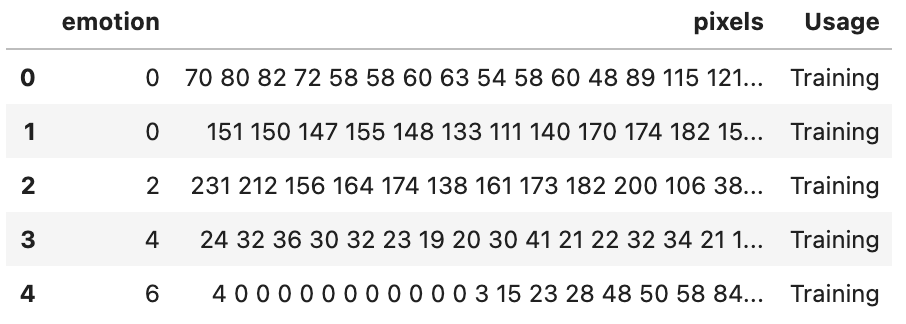
\includegraphics[scale=0.3]{Data}\
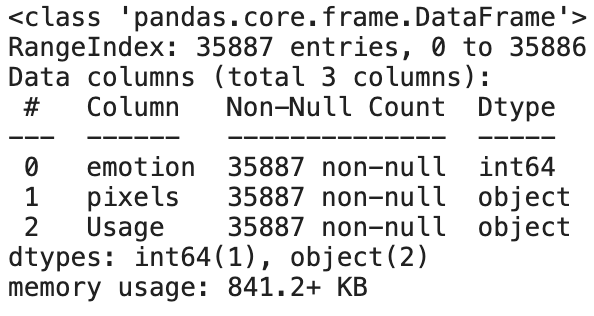
\includegraphics[scale=0.3]{Data1}
\captionof{figure}{Database shape}
\label{fig7}
\end{center}

In order to process our data we have not made a data increase. In our database (FER 2013) the images were already in the right format, in the right direction and in the right colors.


\subsection{Results}

For this project, we did not use a GPU because our computers did not have the appropriate graphic card to use it. Using a GPU would have saved us time in compiling the model, but would not have changed the results.\\

The final test accuracy of our model is about 56\% to 57\% of training accuracy.
It may be not very high like that, but it works and we will explain why we have not managed to increase this number.

\begin{center}
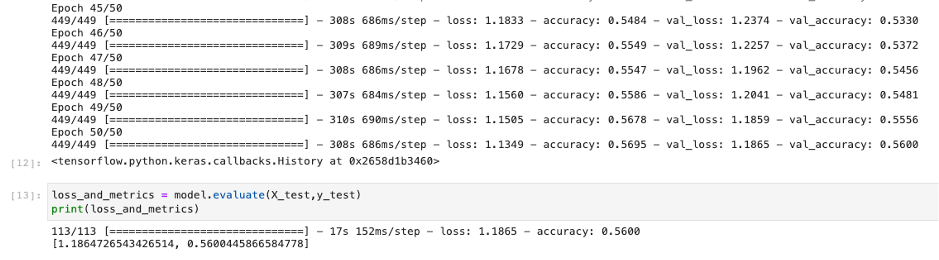
\includegraphics[scale=0.55]{Results}
\captionof{figure}{Model Results}
\label{fig8}
\end{center}

To increase the accuracy, we tried to train more our model with a lot of epochs, but we came in an overfitting.
Indeed, we made a test with 100 epochs.
The training accuracy rose up to 90\% , but the test accuracy stagnates about 59 \%.
This is the sign of an overfitting model and during the test with our webcam we have noticed that this model was very disorienting and stayed on one or two emotions, no matter the face we made.
So, after that, when we check the evolution of the accuracy, we have noticed that the test accuracy value stagnates nearby 55-56\% already at 40 epochs and don’t rise so much after that.
So the model that we use finally is a model training during 50 epochs with 56\% accuracy, and we noticed it’s enough for the test on our webcam, the model run correctly.

\begin{center}
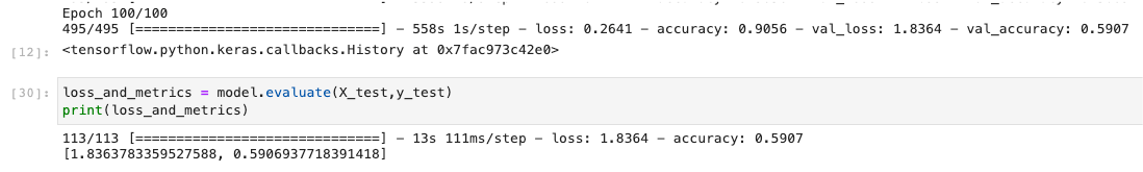
\includegraphics[scale=0.45]{Bad_Results}
\captionof{figure}{Overfitting}
\label{fig9}
\end{center}

The next picture shows the evolution of the training accuracy and the validation accuracy according to the epochs.
We can see that the validation accuracy is near by the training accuracy all the long of the 50 epochs so it illustrates the fact that we don't have overfitting like we explain above.

\begin{center}
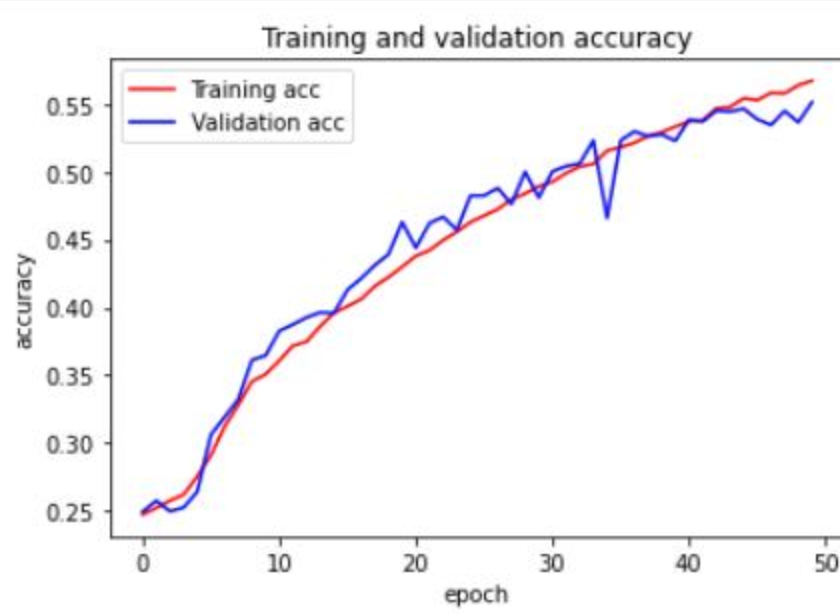
\includegraphics[scale=0.5]{Graph_training_test}
\captionof{figure}{Training \& validation accuracy graph}
\label{fig10}
\end{center}


Then, on the figure 11 is the confusion matrix.
Like the validation accuracy, the results are not perfect, but it works and we are in the same range of results as other works using the same database.


\begin{center}
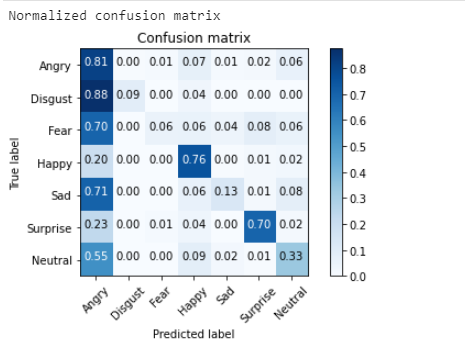
\includegraphics[scale=0.7]{Confusion_matrix}
\captionof{figure}{Confusion matrix}
\label{fig11}
\end{center}


We have seen it has some difficulties to predict the "disgust" emotion.
To fix that we can improve our training model or take another database.
For example, during our research we find many databases for the emotion recognition like:
\begin{itemize}
\item Google Facial Expression Comparison Dataset
\item EMOTIC
\item Dreamer
\item AffectNet
\end{itemize}
\

And a nice improvement, we thought about is to add the reading of the body language to the reading of the emotion of the face.


%%%%%%%%%%%%%%%%%%%%%%%%%%%%%%%%%%%%%%%%%%%%%%%%%%%%%%%%%%%%
\section{DISCUSSION AND CONCLUSION}
In conclusion, this emotion recognition programme is already working very well.
Indeed, we can easily detect most of the emotions, which proves the success of our program. 
Finally, we will conclude with some ameliorations for the application.
First, as explained above in the result point, we can make some improvements to improve the detection of the disgusted emotion.
Secondly, the expression of the body can help to identify the global emotion of a person.
As we can see with the example with Serena Williams, we may not detect if her face is happier or fear, but if we look at her body language, we can say that it is a happy behaviour due to the win.

\begin{center}
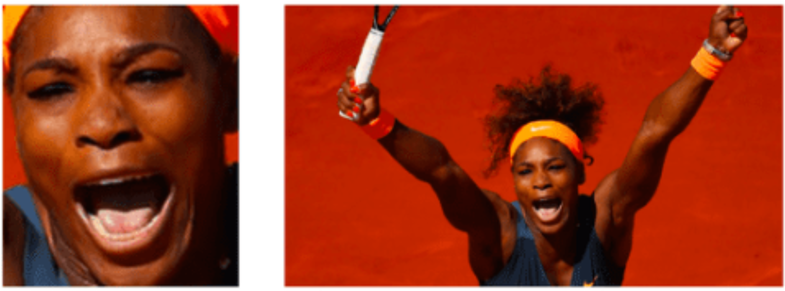
\includegraphics[scale=0.5]{Williams}
\captionof{figure}{Serena Williams emotion}
\label{fig12}
\end{center}

%%%%%%%%%%%%%%%%%%%%%%%%%%%%%%%%%%%%%%%%%%%%%%%%%%%%%%%%%%%%

\begin{thebibliography}{99}

\bibitem{c1}
S.Gharsalli : "Reconnaissance des émotions par traitement d’images". https://tel.archives-ouvertes.fr/tel-01622639/document

\bibitem{c2}
Priya Dwiveldi : "Face Detection, Recognition and Emotion Detection in 8 lines of code!". https://towardsdatascience.com/face-detection-recognition-and-emotion-detection-in-8-lines-of-code-b2ce32d4d5de

\bibitem{c3}
Priya Dwiveldi : "face\_and\_emotion\_detection". https://github.com/priya-dwivedi/face\_and\_emotion\_detection

\bibitem{c4}
Rohit Dwivedi: “My first CNN project – Emotion Detection Using Convolutional Neural Network With TPU”.  https://analyticsindiamag.com/my-first-cnn-project-emotion-detection-using-convolutional-neural-network-with-tpu/

\bibitem{c5}
Sampriti ChatterJee (Great Learning) : “Emotion Detection using Python Convolutionnal Neural Network” https://www.youtube.com/watch?v=m0fWjP3yIEo

\bibitem{c6}
Kaggle : “Facial Expression Recognition Challenge – FER 2013”  https://www.kaggle.com/msambare/fer2013

\end{thebibliography}

\listoffigures

\end{document}
